\documentclass[11pt]{beamer}
\usetheme{PaloAlto}
\usecolortheme{seahorse}
\usepackage[utf8]{inputenc}
\usepackage{amsmath}
\usepackage{amsfonts}
\usepackage{amssymb}
\usepackage{graphicx}
\usepackage{animate}
\usepackage{textpos}

\graphicspath{{./figures/}}
%\graphicspath{{C:\Users\Jeroen Frans\Documents\Projects\Demo-HDR\figures\}}
\author{Jeroen}
\title{Git with a GUI}
\setbeamercovered{transparent} 
\setbeamertemplate{navigation symbols}{} 
\logo{\includegraphics[height=1.4cm]{Hedera_logo.png}} 
%\institute{} 
%\date{} 
%\subject{} 
\begin{document}

\begin{frame}
\titlepage
\end{frame}

%\begin{frame}
%\tableofcontents
%\end{frame}

\section{Wat is Git?}
\begin{frame}{Principe achter Git}
\begin{itemize}
\item Versie Controle
\item Historiek van code
\item Geen centrale server (CVS, SVN)
\end{itemize}
\hspace{200pt}
\includegraphics[scale=.2]{git-icon.png}
\end{frame}

\begin{frame}{CLI vs GUI}
Git kan gebruikt worden vanuit Command Line Interface (\textbf{CLI})\\
$\Rightarrow$ Zie cursus op dataCamp\\
\vspace{12pt}
Alternatief kan een \textbf{GUI} gebruikt worden:
\begin{itemize}
\item GitKraken (Windows, Mac en Linux)
\item SourceTree (Windows en Mac)
\item \dots
\end{itemize}
\end{frame}

\section{Waarom Git?}
\begin{frame}{Waarom Git?}
\emph{1. Voor jezelf:}
\begin{itemize}
\item Terugkeren naar historische versie van code
\item Brengt structuur in je werk
\end{itemize}
\emph{2. Voor je team:}
\begin{itemize}
\item \textbf{Git Flow}
\item Combineren met Kanban Board
\item Parallel programmeren
\end{itemize}
\emph{3. Voor je klant:}
\begin{itemize}
\item Transparantie van de hele analyse
\item Agile
\end{itemize}
\end{frame}

\section{Principes}
\begin{frame}{Centrale concepten}
\begin{itemize}
\item Staging \& commiting
\item Branching
\item Remote repositories (Github)
\item Collaboratie met git
\item Git Flow en agile projecten
\end{itemize}
\end{frame}

\subsection{Staging \& Commiting}
\begin{frame}{Staging}
Git gaat een map op je computer volgen en tracken wat er gewijzigd wordt. Het doet dit echter enkel voor bestanden die jij vastlegt.\\
\vspace{8pt}
Dit klaarzetten om veranderingen op te slaan heet \textbf{staging}. Het alternatief is een bestand tijdelijk niet klaar te zetten of het volledig negeren door het in het '\textit{.gitignore}' bestand te zetten.\\
\vspace{8pt}
In CLI $\rightarrow$ git add [file]
\end{frame}

\begin{frame}{Commits}
\begin{itemize}
\item Eenmaal staged $\Rightarrow$ klaar voor commit
\item Persistent wegschrijven
\item Krijgt hash toegewezen (belangrijk in CLI)
\end{itemize}
\center
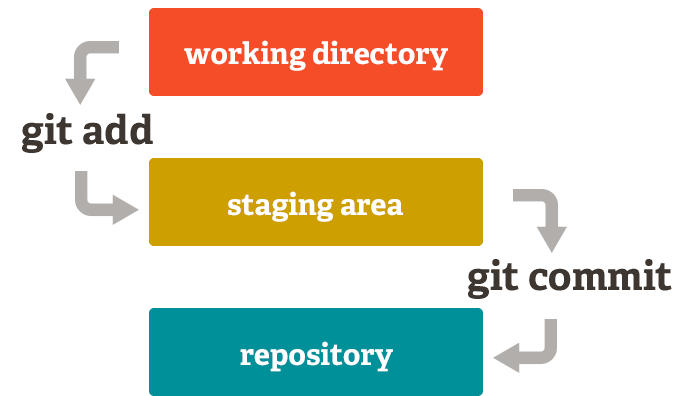
\includegraphics[scale=.25]{git_staging_commit.png}
\end{frame}

\subsection{branching}
\begin{frame}{Branches}
Het is mogelijk om parallel meerdere stukken code te ontwikkelen. Hiervoor moet je een 'kopie' van je code maken van waaruit je verder kan ontwikkelen.\\

\begin{itemize}
\item Creëer een branch
\item Probeer naam inhoudelijk overeen te laten stemmen met doel
\item Als de ontwikkeling klaar is, laat je deze branch terug samenkomen met de hoofdtak = \textit{merging}
\item Hierdoor kunnen mogelijk conflicterende bestanden ontstaan
\end{itemize}
\end{frame}

\begin{frame}{Merging}
Als je twee branches samenvoegt, gaat git de verschillen tussen de twee branches zoeken. \\

\center
%\animategraphics[loop,controls,width=120pt]{30}{merge-}{0}{144}
\end{frame}


\end{document}